\documentclass[10pt,conference,compsocconf]{IEEEtran}

\usepackage{hyperref}
\usepackage{graphicx}	% For figure environment

% Packages added by Joachim

%drow graph
\usepackage{fancybox}
\usepackage{tikz}
\usepackage{capt-of}
\usepackage{verbatim}

% cancel math expression
\usepackage{cancel}

% math
\usepackage{amsmath}

% math symbols
\usepackage{amssymb}

% url
\usepackage{url}

%subfigure
\usepackage{subcaption}
\usepackage{cleveref}

% multiline tabular cell
\newcommand{\specialcell}[2][c]{%
  \begin{tabular}[#1]{@{}l@{}}#2\end{tabular}}
  
% nice fraction
\usepackage{units}


\usepackage[export]{adjustbox}% http://ctan.org/pkg/adjustbox



\begin{document}

%\AddToShipoutPictureBG{%
%  \AtPageUpperLeft{\raisebox{-\height}{
\includegraphics[width=1.5in]{img/Dori}}}%
%}

\title{PCML CS-433: Recommender System}

\author{
  %Team: {\bsifamily \large ``Just keep swimming !''} {\hspace{0.1cm} 
\includegraphics[width=0.3in ,valign=t]{img/Dori}} \\ \\
   \hspace{0.8cm} Team: {
\includegraphics[width=2.5in ,valign=t, trim=0cm 0 0 3.8cm]{img/Dory.png}} \\

  %Team: {\bf Netflix and MaCHILL Learning} \\
  Gael Lederrey, SCIPER 204874, gael.lederrey@epfl.ch \\
    Joachim Muth, SCIPER 214757, joachim.muth@epfl.ch\\
  Stefano Savar\`e, SCIPER 260960, stefano.savare@epfl.ch \\
 \\ 

  \textit{School of Computer and Communication Sciences, EPF Lausanne, Switzerland}
}

\maketitle

%========================
\begin{abstract}
Active Collaborative Filtering Recommender Systems for movie collection using blending of 30 different methods (8 direct scoring methods\footnote{means, medians, ...} and 9 iterative ones, plus 13 variations of them) in order to achieve around 0.97452
 RMSE on Kaggle's EPFL ML Recommender System challenge. 
\end{abstract}

%========================
\section{Introduction}

Collaborative filtering is a set of techniques aiming at the creation of recommender systems. Usually, we define three types of collaborative filter: \textbf{active}, \textbf{passive} and \textbf{content-based} (the best one being obviously a mix of the three). In industry, recommenders are mainly used to suggest new item to users based on their taste: movies, music tracks, items to purchase, ...

The objective of the project is to develop a recommender system using \textbf{active collaborative filtering} (i.e. pseudonymised items\footnote{Items anonymized by an ID, i.e. we have access neither to the name nor any content of it.} rated by pseudonymised users).

We first go through a general \textbf{data analysis} in order to evaluate the quality of the data (spammers and participation of the users). Then we test different models, starting from a basic mean given a prediction baseline and improving the score with more advanced algorithms.

According to \textit{BellKor's Pragmatic Chaos}\footnote{Winner team of 2009 Netflix Prize} scientific paper \cite{BellKore_netflix} the best recommender is obtained through a clever blend of several models. Exploiting this approach, \textbf{we ultimately blended 30 different methods (8 direct scoring methods and 9 iterative ones, plus 13 variations of them)} eventually achieving around 0.95962 RMSE on local Cross-Validation (0.97452 on Kaggle test set).

The implemented model will be part of the \textbf{Kaggle's EPFL ML Recommender System} challenge in which predictions are rated by their RMSE compared with ground truth values. All external libraries are allowed as long as they are properly documented.

%========================
\section{Data Description}

The data represent ratings from $10'000$ users on $1'000$ movies in an integer scale from 1 to 5. Both of them are pseudonymized by an ID. This scale represents the number of \textit{stars} given by the users, 1 being the lowest grade and 5 the best.

The training set used to train our algorithm contains $1'176'952$ ratings which represent around 12\% of filled ratings. 
Another $1'176'952$ ratings are hidden from us and must be predicted by our recommender algorithm in order to be scored on Kaggle platform.


%\begin{figure}[htbp]%------- PICTURE---------
%  \centering
%  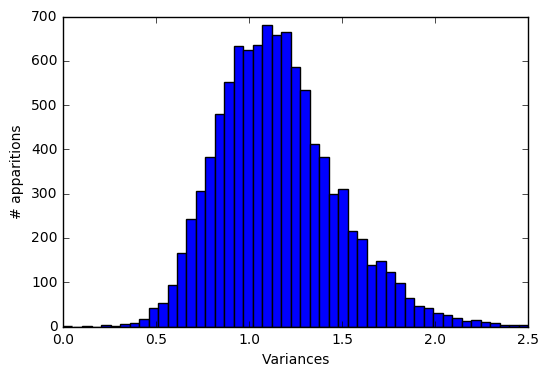
\includegraphics[width=0.9 \columnwidth]{img/Variances}
%  \caption{Distribution of variances of ratings per user.}
%  \vspace{-3mm}
%  \label{fig:denoise-fourier}
%\end{figure}
%\begin{figure}[htbp]
%  \centering
%  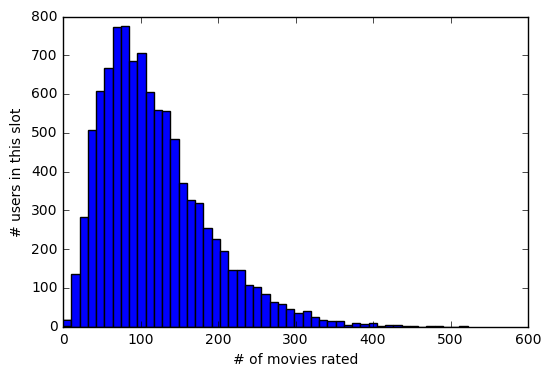
\includegraphics[width=0.9 \columnwidth]{img/Ratings}
%  \vspace{-3mm}
%  \caption{Number of movies rated per user.}
%  \label{fig:denoise-wavelet}
%\end{figure}


\begin{figure}[tbp] %-------------- FIGURE -------------
    \centering
    \hspace{-0.6cm}
    \begin{subfigure}[t]{0.45\columnwidth}
        \centering
        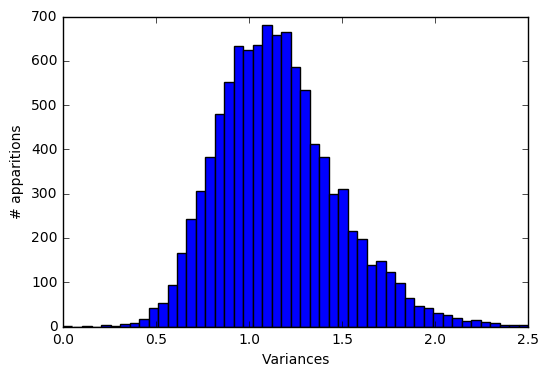
\includegraphics[height=1.2in]{img/Variances}
        \vspace{-3mm}
  \caption{Distribution of variances of ratings per user. No spammers.}
  \label{variances}
    \end{subfigure}%
    \hspace{0.4cm}
    \begin{subfigure}[t]{0.45\columnwidth}
        \centering
        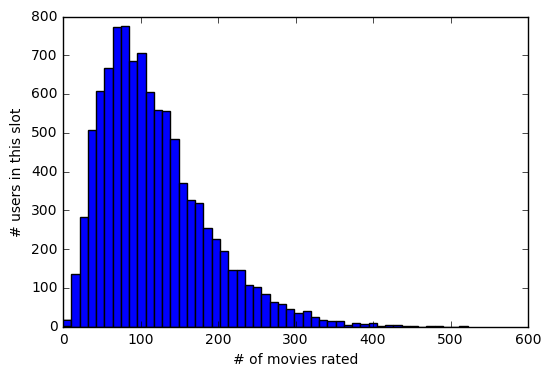
\includegraphics[height=1.2in]{img/Ratings}
        \vspace{-3mm}
        \caption{Number of movies rated per user. Good user participation.}
        \label{number_ratings}
    \end{subfigure}
    \caption{Statistical description of the data}
\end{figure}


%========================
\section{Data Exploration}

\subsection{Search for Spammers}

One of the first step before starting learning from data is to ensure that they are real ones, and not produced by bots (spammers). As we know, spammers can act in different ways: \textbf{uniform spammers} constantly rate movies in the same way, while \textbf{random spammers} randomly rate movies. Figure (\ref{variances}) shows the Gaussian distribution of the rating variances and ensure the data are free of spammers.

\subsection{Participation of Users}

Even free of spammers, data can still contain \textbf{inactive users}, i.e. users who subscribed to a platform but never use it or never rate movies. If they are in too big number compared with active users, they can disturb learning algorithms. Figure (\ref{number_ratings}) shows histograms of number of movies rated by users and confirm us the good participation of the users.

\subsection{User "Moods" (Deviation)}

Because of mood/education//habits \textbf{users having the same appreciation of a movie can rate it differently}. Indeed, we show in the figure (\ref{mood}) that some users systematically rate lower/higher than others. It's interesting to take this effect into account to create a variation of a model. (see section \ref{choice_model}).

\begin{figure}[htbp] %-------------- FIGURE -------------
  \centering
  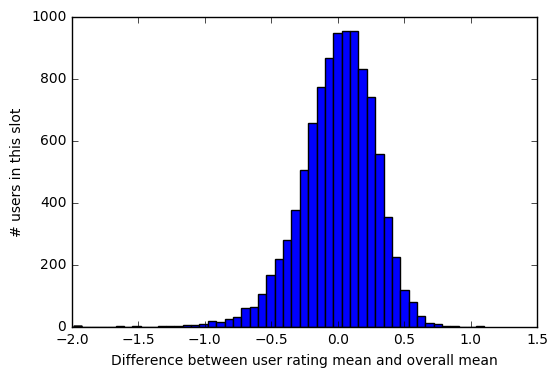
\includegraphics[width=\columnwidth]{img/Deviation_mean}
  \caption{Difference of rating mean of each user compared with overall mean. Illustrates the differences of judgement that users give in average or what we call in this paper the "moods".}
  \vspace{-3mm}
  \label{mood}
\end{figure}

%========================
\section{Models}

\subsection{Global mean/median (2 models)}

The simplest model is to take all the ratings in the train set and apply the mean or the median value. We return this value as the prediction. This give a baseline score from which we can compare further models.

\subsection{User/Movie mean/median (4 models)}

Another simple model is to compute the mean or median value for the users or the movies.

\subsection{Movie mean/median with normalized user moods (2 models)}

The third set of model uses the mean or median value for each movie. We also compute the ``mood'' of the users this way:

\begin{equation}
 d_u = \overline{U} - \overline{u} \quad \forall u\in U
\end{equation}
where $\overline{U} = \frac{1}{\#U} \sum_{u\in U} \overline{u}$ and $\overline{u}$ being the average rating of the user $u$.

Then, we return the prediction of a user $u$ on a movie $m$:
\begin{equation}
 p_{m,u} = \overline{m} + d_u
\end{equation}
where $\overline{m}$ is either the mean or the median of the ratings on the movie $m$.

\subsection{Matrix Factorization using Stochastic Gradient Descent (MF-SGD)}
\label{sec:mf-sgd}
Given $D$ items, $N$ users and the corresponding rating matrix 
$X \in \mathbb{R}^{D \times N}$, we aim to find two matrices $W \in \mathbb{R}^{D \times K}$ and $Z
\in \mathbb{R}^{N \times K}$ such that the quantity 

\begin{multline}
\label{eq:functional}
E = \frac{1}{2} \sum_{\substack{d=1,...,D \\n=1,...,N}} 
\bigg( x_{dn} - \big( WZ^T \big)_{dn} \bigg) ^2 + \\ 
\frac{\lambda}{2}\|W\|^2 + \frac{\lambda}{2}\|Z\|^2
\end{multline} 

is minimized. $K$ is a parameter,
corresponding to the number of the \textit{latent factors}; $\lambda$ is a scalar 
that weight the regularization terms.

The Stochastic Gradient Descent method is a faster variant of the standard gradient descent
optimization. The gradient of the functional \ref{eq:functional} is computed only on a single
element of the summation, randomly chosen. The update process then follows the same rules of the batch
gradient descent.
An almost certain convergence to a local minimum is guaranteed under not restrictive hypothesis.

\subsection{Matrix Factorization using Alternating Least Square (ALS)}
ALS is one of the main alternatives to the SGD to solve problem \ref{eq:functional}.
It is an iterative algorithm consisting in alternately fixing one of the two matrices $W$ or $Z$,
while optimizing the problem \ref{eq:functional} with respect to the other matrix.
The optimization problem at each iteration is much easier to solve compared to the one solved by the
SGD. A simple least squares technique can be exploited.

%For speed reasons we decided to use the open source framework Apache Spark to implement this method.
PySpark\footnote{Apache Spark Python wrapper} provides the library \texttt{pyspark.mllib.recommendation.ALS}. It
is a cluster computing framework that provides to the programmers an application programming
interface to efficiently execute streaming, machine learning or SQL workloads that require fast
iterative access to datasets.

\subsection{PyFM}

%We implemented two version of the SGD methods:
%\begin{itemize}
%\item An implementation from scratch, using \texttt{scipy.sparse} matrices library.
%\item An implementation based on the PyFM Python library, a wrapper of the C++ library libFM
%\cite{rendle:tist2012}, one of
%the most advanced matrix factorization libraries.
%\end{itemize}

PyFM is a python implementation of Factorization Machines. This library is a wrapper of the C++ library libFM \cite{rendle:tist2012} and can be found on Github \cite{pyfm}. The idea behind the algorithm is similar to the MF-SGD. 

\subsection{Matrix Factorization using Ridge Regression (MF-RR)}

\subsection{Baseline}

\subsection{Slope One}

\subsection{SVD}

\subsection{KNN item/user based}


%========================
\section{Blending}
\label{sec:blending}

The \textit{Bellkor's Pragmatic Chaos} team, winner of 2009 \textit{Netflix Prize}, explain in its paper that its solution was obtained by blending a hundred different models. \cite{BellKore_netflix} Without having the same number of models, we proceed the same to obtain our final solution. We perform a weighted sum that we optimize using \textbf{Sequential Least Squares Programming} (SLSQP) method provided by \texttt{scipy.optimize.minimize} library. Initial weights are set to $\nicefrac{1}{n}$ for each model ($n$ being the number of models). Instead of constraining the weights to be between 0 and 1, and to have a sum equal to 1, we choose to let the optimizer have more flexibility.

\subsection{SLSQP method}
\label{SLSQP}
Sequential Least Squares Programming method is a \textbf{Quasi-Newton method}. Unlike Newton method, it does not compute the Hessian matrix but estimates it by successive gradient vector analyze \cite{wiki:quasi_newton} using \textbf{Broyden-Fletcher-Goldfarb-Shanno} algorithm (BFGS). This method allows optimization for function without knowing Hessian matrix, in a short computation time.

\begin{table}[htbp]
\centering
\begin{tabular}[c]{| l r |}
\hline
Model & RMSE \\
\hline 
\hline
Global Mean                  	           			& 1.11905\\
Global Median                          			 	& 1.12811\\
User Mean                               				& 1.09516\\
User Median                             				& 1.15146\\
Movie Mean                              				& 1.03043\\
Movie Mean Rescaled                    			& 1.00562\\
Movie Median                            				& 1.09968\\
Movie Median Rescaled                  			& 1.02267\\
Movie Median Deviation User           			& 1.07220\\
Movie Median Deviation User Rescaled 		& 1.06465\\
Movie Mean Deviation User             			& 0.99661 \\
Movie Mean Deviation User Rescaled   		& 1.04494\\
MF RR                                   				& 1.02774\\
MF RR Rescaled                         			& 1.02746\\
MF SGD                                  				& 1.00080\\
MF SGD Rescaled                       			& 0.99993 \\
ALS                                      				& 0.98874\\
ALS Rescaled                           				& 0.98903 \\
PyFM                                     				& 0.98802 \\
PyFM Rescaled                           			& 0.98863 \\
Baseline                                 				& 0.99925 \\
Baseline Rescaled                       			& 1.00039\\
Slope One                               				& 1.00010\\
Slope One Rescaled                     			& 1.00032\\
SVD                                      				& 0.99835\\
SVD Rescaled                            			& 0.99840 \\
KNN Item Based                                  		& 0.99031 \\
KNN Item Based Rescaled                        		& 0.99043\\
KNN User Based                                  		& 0.99244 \\
KNN User Based Rescaled                       		& 0.99351 \\
 \hline \hline
Blending			&  0.95962 \\ 
\hline
\end{tabular}
  \caption{Benchmark of models.}
  \label{benchmark}
\end{table}


%========================
\section{Result}

In order to create our recommender algorithm, we followed the steps: 
\begin{enumerate}
\item \textbf{Tuning the parameters} for each model one-by-one following a grid-search method scored by a 5-fold Cross-Validation. 

\item \textbf{Computing the predictions} for each model for 5 folded set of data. This result to a set of $5n$ prediction tables\footnote{$n$ being the number of models} that can be tested agains 5 validation tables, providing 5-fold Cross-Validation.

\item \textbf{Optimizing the weights} for each model prediction produced by the previous step, by running a SLSQP optimization method (as explained in section \ref{SLSQP}) on the 5 folded prediction tables.
\end{enumerate}


% ==============================
\subsection{Benchmark}
\label{sec:model_bench}

Table \ref{benchmark} presents the average RMSE of each model applied on the validation sets for the blending cross validation process. Last line is the result of the blending on the same validation sets.


The blending gives a 0.97452 RMSE on Kaggle's test set. 


% ===================================================
\subsection{Blending}

Table \ref{blending} provides the weights after optimization. It also provides the parameters used for each model.

%===================================
\begin{table}[htbp]
\centering
\begin{tabular}[c]{| l r l |}
\hline
Model 				& Weight 							& Parameters\\
\hline 
\hline

Global Mean                  	           			& 1.77567		 			& - \\
Global Median                          			 	&1.84693					& - \\
User Mean                               				& -3.64246					& -\\
User Median                             				& 0.00513					& -\\
Movie Mean                              				& -0.83307					& -\\
Movie Mean Rescaled                    			& -0.95695					& -\\
Movie Median                            				& -0.93869					& -\\
Movie Median Rescaled                  			& -0.91347					& -\\
Movie Median Deviation User           			& 0.93849					& -\\
Movie Median Deviation User Rescaled 		& 0.96461					& -\\
Movie Mean Deviation User             			& 1.04428					& -\\
Movie Mean Deviation User Rescaled   		& 0.92108					& -\\
MF RR                                   				& 0.03222					& \specialcell[t]{features = 20 \\
																$\lambda = 19$}\\
MF RR Rescaled                         			& 0.03537					& \textit{(idem)}\\
MF SGD                                  				& -0.78708					& \specialcell[t]{$\gamma = 0.004$ \\
																features = 20 \\
																iter = 20 }\\
MF SGD Rescaled                       			& 0.27624					& \textit{(idem)}\\
ALS                                      				& 0.30659					& \specialcell[t]{$\lambda = 0.081$ \\
																rank = 8 \\
																iter = 24}\\
ALS Rescaled                           				& 0.31745					& \textit{(idem)}\\
PyFM                                     				& 0.15296					& \specialcell[t]{features = 20 \\
																iter = 200 \\
																$ \gamma = 0.001$}\\
PyFM Rescaled                           			& -0.02162					& \textit{(idem)}\\
Baseline                                 				& -0.70720					& -\\
Baseline Rescaled                       			& -0.56908					& -\\
Slope One                               				& -0.02311					& -\\
Slope One Rescaled                     			& 0.43863					& -\\
SVD                                      				& 0.67558					& \specialcell[t]{$\gamma = 0.001$,\\
																$\lambda = 0.001$, \\
																iter = 30}\\
SVD Rescaled                            			& -0.00498				& \textit{(idem)}\\
KNN Item Based                                  		& -0.09500				& \specialcell[t]{$k = 60$,\\
																sim. metric = \\
																	Pearson Baseline}\\
KNN Item Based Rescaled                        		& 0.34178					& \textit{(idem)}\\
KNN User Based                                  		& 0.21758					& \specialcell[t]{$k = 300$,\\
																sim. metric = \\
																	Pearson Baseline}\\
KNN User Based Rescaled                       		& 0.12803					& \textit{(idem)}\\



\hline

\end{tabular}
  \caption{ Blending of models. {\footnotesize Legends:  $\gamma$: learning rate, $\lambda$: regularization factor, \textit{idem}: always refers to directly previous model}}
  \label{blending}
\end{table}

%========================
\section{Discussion of the results}

Excluding the trivial models based on the user/movie mean/median, we mainly focused on \textbf{Matrix
Factorization algorithms}, exploiting different techniques to achieve the best factorization
possible. 

Blending plays an important role in our project. As we can see in table \ref{benchmark}, while models rarely score under $0.99$, blending achieve around $0.96$ RMSE. This is explained by the fact that certain model can compensate others for certain kind of users. The role of the optimizer is to find how to combine them in order to achieve best prediction.

%We can first discuss about the models. The models we used are quite simple. Therefore, using more
%complex algorithms instead of these would help in achieving better results. However with our blending method, we can use as many algorithms as we want. Indeed, since we're using an optimization algorithm, the optimization can decide itself if it should discard a model or not. However there's some risk to overfit the data. And it is happening a little bit. Indeed, the RMSE on the validations sets is a bit smaller than the RMSE on Kaggle. 

% =====================================
\subsubsection{Choice of the models}
\label{choice_model}

It should be legitimate to ask \textbf{why we are keeping both normalized and unnormalized model for
some models}. Looking at the coefficients gives a partial answer. As we see in table \ref{blending}, normalized and unnormalized models oppose themselves almost exactly, with a little advantage for normalized models. The effect is that the method is more taken into account for users in the tail of the Gaussian deviation curve (figure \ref{mood}) than for the central ones. Then, it allows the optimizer to have finer control on the blending.

%\subsubsection{Blending Choices} 
%\textcolor{red}{REVIEW}
%The role of the blending part is extremely important in obtaining the best score possible. The large
%number of models available would be pointless without a good blend. Moreover, we mainly consider
%simple models, leaving to the blender the task of building a more complex one.
%
%As mentioned in Section \ref{sec:blending} we used the Sequential Least Square Programming method to
%optimize the weighted sum of models. Simpler methods, like a grid search, are computationally too
%expensive and less accurate than the algorithm used. We spent some time in finding the best
%optimization method for our purposes. \textcolor{red}{review}
%
%%We decided to also allow negative weight. This choice was made for two reasons:
%The optimization choice also allows negative weights. We decided not to put any constraint about that
%for two reasons:
%\begin{itemize}
%\item We obtained better results.
%\item Negative weights may help in better fitting the distribution of the training dataset. This can
%lead to overfitting, as we discuss in the next subsection, but, at the same time, it also produces
%better results.
%\end{itemize}
%We also did not put any constraint on the sum of the weight (i.e. the sum is not fixed  to 1) for the
%same reasons.

\subsubsection{Overfitting}
We apply several techniques to reduce as much as possible the overfitting of the models we used. In
particular we used a \textbf{5-fold cross-validation both to determine the best parameters for each model and to
choose the best weights in the blending.}
Despite this, the model slightly overfits the data. With a 0.95962 RMSE on our local Cross-Validation and 0.97452 on Kaggle's test set, we notice a small difference that indicates overfitting.

There are many possible reasons underlying this behaviour. Probably the blending process that we
used, although the proven accuracy, introduces too much complexity in the model, thus overfitting
the training database.





\bibliographystyle{IEEEtran}
\bibliography{literature}

\end{document}
